\chapter{Rapport intérmédiaire : 17.09.2018 au 12.10.2018}

Ce premier résumé a pour but de poser le projet et d'étudier l'état de l'art. Depuis les lectures concernant ce qu'il existe en machin learning pour le positionnement indoor, il est nécessaire de faire un résumé afin de choisir le meilleur algorithme afin d'améliorer le positionnement indoor à l'aide de la technologie LoRa et le mode ranging.

\section{Cahier des charges}
\subsection{Introduction}
Les systèmes de localisation basés sur GPS souffrent de la détérioration de la précision et sont presque indisponibles dans les environnements intérieurs. Pour les environnements intérieurs, de nombreuses technologies de systèmes de positionnement ont été conçues sur la base de la vision, de la détection infrarouge ou ultrasonore, des champs magnétiques de la terre, des accéléromètres / gyromètres, des balises BLE ou de la communication WiFi. Chacune de ces technologies existantes a des coûts, une précision et un compromis maximum en matière de couverture, mais un service de localisation intérieur générique reste difficile à obtenir.

\subsection{But du projet}
S'appuyant sur les capacités étendues des nouveaux circuits intégrés LoRa, ce projet développera et déploiera un système de localisation capable d'améliorer la précision de la position atteinte par les systèmes de localisation basés sur LoRa existants reposant sur des mécanismes TDOA ou de télémétrie. À cette fin, une exploration et une comparaison des différentes techniques "machine learning/deep learning" pour le positionnement basé sur le "fingerprinting" seront effectuées.


\subsection{Objectifs et tâches à réaliser}
\begin{enumerate}
	\item Etudier le cahier des charges
	\item Etudier l’état de l’art des techniques à utiliser dans le cadre du projet, en particulier les systèmes de localisation indoor basés sur des techniques d’apprentissage, et réunir une documentation (env. 20% effort)
	\item Etablir un planning pour l’ensemble du projet.
	\item Définir un plan des tests à effectuer.
	\item Définir les procédures de test
	\item Définir le setup pour la collecte de données de localisation
	\item Prise en main de l’environnement de développement pour les phases de training et du test de la technique d’apprentissage retenue (e.g., PyTorch).
	\item Implémentation de la solution ML retenue.
	\item Tester le système selon le protocole préétabli.
	\item Faire des propositions pour améliorer les performances de l’algorithme et, si possible, les implémenter.
	\item Rédiger le rapport et documenter l’ensemble du projet.
\end{enumerate}


\section{Résumé du document 00}
Ce document décrit la localisation sans utiliser le GPS et en utilisant LoRa. Il a surtout été utile d'utiliser ce document pour la gestion des "outliers"
\\
\\
Le problème principal avec le GPS c'est la consommation et la durée de vie c'est pourquoi un système basé sur LoRa a été étudié. La portée en milieu rural est d'environ 15km alors qu'il est de 5km dans un milieu urbain cela grâce à la bonne sensibilité du récepteur (-130dBm). Une chose intéressant est la bande passante qui est plus large que d'autres technologies qui permet de distinguer différents chemins du même signal. Sagemcom ont obtenus des bons résultats au niveau de la précision qui est de environ 4 mètres. 
\\
\\
Ce qui est intéressant c'est dans cette publication c'est la manière de traiter les "outliers - valeurs aberrante, c'est-à-dire les points qui ne sont pas cohérent lors d'une mesure. Selon Barnet et Lewis [11], un "outliers" est définit comme étant une observation qui semble incompatible avec le reste d'un ensemble de données.
Garder un "outliers" dans une set de données peut amener à de mauvais résultat il est donc important de les détecter correctement. Il existe différentes méthodes pour déterminer ces "outliers" :

\begin{enumerate}
	\item Grubbs' test : Détecte un "outliers" en supposant une distribution normale.
	\item Tietjen-Moore test : C'est une généralisation de Grubbs' test pour détecter de multiple outliers. Il a cependant un inconvénient, il est nécessaire de connaitre le nombre exact d'ouliers.
	\item Generalized Extreme Studentized Deviate (ESD): C'est également une généralisation du test Grubbs' mais il n'est pas nécessaire de connaitre à l'avance le nombre d'ouliers. Ce test nécessite uniquement une limite supérieure pour le nombre suspect d'outliers.[01]
\end{enumerate}

[11] V. Barnett; T. Lewis, Outliers in Statistical Data, 3rd ed. Wiley Series in Probability and Mathematical Statistics, 1994.

[01] lien concernant les ESD : https://www.itl.nist.gov/div898/handbook/eda/section3/eda35h3.htm

\section{Résumé du document 01}
Cette publication parle d'une analyse comparative entre différents algorithmes de "machine learning" pour du positionnement indoor. L'étude est basée sur un positionnement "fingerprint" ce qui permet de cartographier un endroit à l'aide du de la force du signal récéptionné (RSS - Received Signal Strength).
Dans cet article, les algorithmes de "machine learning" sélectionnés sont comparés en termes de précision de positionnement et de temps de calcul. la base de donnée UJIIndoorLoc a été utilisé pour les différentes expérimentation. Les résultats expérimentaux révèlent que l’algorithme k-Nearest Neighbor (k-NN) est le plus approprié lors du positionnement.

\subsection{Introduction}
Au cours des expériences, la base de données UJIIndoorLoc, qui est préparée pour les systèmes de positionnement à l'intérieur [8], est utilisée. La classification est effectuée en premier lieu en utilisant le jeu de données d'origine en considérant les valeurs RSS de 520 points d'accès sans fil (WAP) et les nouveaux attributs définis en tant que «cellule» qui composent les attributs BuildingID, Floor, SpaceID et RelativePos. Ensuite, une nouvelle méthode est proposée: «Séparation déductive pour le positionnement intérieur (DESIP - Deductive Separation for Indoor Positioning)». Dans cette méthode, tout d'abord, seules les informations de bâtiment et les valeurs RSS mesurées à partir de 520 WAP sont utilisées pour la tâche de classification.
\\
\\
Durant les expériences, des algorithmes déterministes tels que le plus proche voisin (NN - nearest neighbor), le SMO, l'arbre de décision (J48) et des algorithmes probabilistes tels que Naïve Bayes et Bayes Net sont utilisés. L’algorithme le plus approprié pour la solution du problème de positionnement intérieur est déterminé en comparant la précision et le temps de calcul de chaque approche.
\\
\\
La base de données entière est séparée de telle sorte que 19.937 enregistrements soient réservés à la formation et 1.111 enregistrements soient réservés aux tests. Il y a 529 caractéristiques et ces caractéristiques sont les coordonnées où sont prises les empreintes digitales WiFi, telles que bâtiment, étage, espace (bureau, laboratoire, etc.), position relative (dans une pièce ou dans un couloir), etc. Le jeu de données de formation UJIIndoorLoc comprenant les valeurs RSS de 520 WAP et un nouvel attribut «cellule» qui compose les attributs floor, buildingID, spaceID et relative position de l'ensemble de données d'origine est utilisé pour la tâche de classification. Les étapes des expériences utilisant ce jeu de données sont illustrées à la figure \ref{fig:newAttribute}.

\begin{figure}[htp]
	\begin{center}
		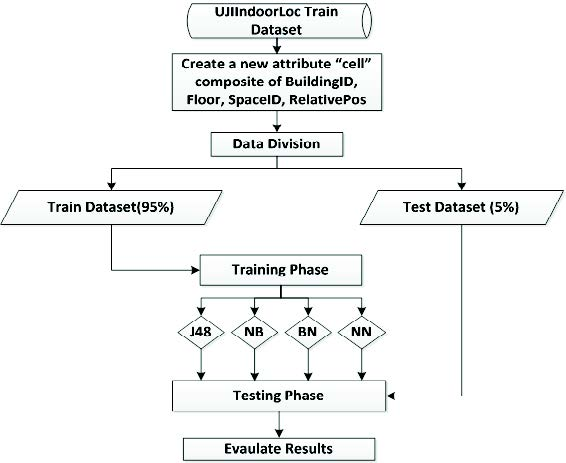
\includegraphics[scale=1]{figures/newattribute.jpg}
		\caption{The new attribute “cell” construction phase}
		\label{fig:newAttribute} %% NOTE: always label *after* caption!
	\end{center}
\end{figure}


\subsection{Algorithmes}
Dans la section suivante, les algorithmes de classification utilisés dans cette étude sont brièvement décrits.

\subsubsection{Decision Tree}
L'arbre de décisions et une méthode très connue en "machine learning". Il possède des noeuds de décisions (non-terminal), des branches, et des noeuds feuilles (terminal) qui représentent les caractéristiques, condition et les classes. A chaque noeud de décision on sait quelle branches suivre et lorsque l'algorithme atteint un noeud final, le label contenu dans ce même noeud est retourné comme étant la classe. 
L’ID3 de Quinlan et son successeur, C4.5, sont les plus populaires parmi les algorithmes d’arbre de décision [19].

(19) J. R. Quinlan, “ C4. 5: programs for machine learning”, Elsevier, 2014.

\subsubsection{Naïve Bayes}
Le classificateur Naïve Bayes [22] basé sur le théorème de Bayes est un algorithme d'apprentissage supervisé [23]. Il est robuste aux données bruyantes, facile à construire, affiche une grande précision et rapidité lorsqu'il est appliqué à de grandes bases de données et exécute des modèles de classification plus complexes. Par conséquent, il est largement utilisé dans les tâches de classification. Il calcule la probabilité de chaque attribut dans les données en supposant qu'elles sont également importantes et indépendantes les unes des autres. Cette hypothèse est appelée indépendance conditionnelle de classe [24, 25].
\\
\\
(22) G. H. John, and P. Langley, “Estimating Continuous Distributions in Bayesian Classifiers”, 11th Conference on Uncertainty in Artificial Intelligence, pp., 338-345, 1995.

(23) C. Anuradha, and S. Dhall, "Software Defect Prediction Using Supervised Learning Algorithm and Unsupervised Learning Algorithm", 2013.

(24) W. Yotsawat, and A. Srivihok, "Inbound tourists segmentation with combined algorithms using K-Means and Decision Tree”, 10th International Joint Conference on Computer Science and Software Engineering (JCSSE), pp.189-194, 2013.

(25) S. Ureerat, and P. Singsri, "The classifier model for prediction quail gender after birth based on external factors of quail egg", IEEE 11th International Joint Conference on Computer Science and Software Engineering (JCSSE), 2014.

\subsubsection{Bayesian Network}
\subsubsection{K-Nearest Neighbor}
\subsubsection{SMO}
\subsubsection{AdaBoost}
\subsubsection{Bagging}


\subsection{Conclusions}

\section{Résumé du document 02}
\subsection{Pro/con}

\section{Résumé du document 03}
\subsection{Pro/con}